% titlepage-demo.tex
\documentclass{beamer}
\usepackage{graphicx}
\usepackage{tikz}
\usepackage{xcolor}
\usetikzlibrary{matrix}
% items enclosed in square brackets are optional; explanation below
\title{Verifying Filesystem Data Structure Properties}
\subtitle{Using a FAT32-like filesystem organisation}
\author{Mihir Mehta}
\institute{
  Department of Computer Science\\
  University of Texas at Austin\\[1ex]
  \texttt{mihir@cs.utexas.edu}
}
\date{06 April, 2018}

\AtBeginSection[]
{
  \begin{frame}<beamer>
    \frametitle{Outline}
    \tableofcontents[currentsection]
  \end{frame}
}

\addtobeamertemplate{navigation symbols}{}{%
    \usebeamerfont{footline}%
    \usebeamercolor[fg]{footline}%
    \hspace{1em}%
    \large \insertframenumber/\inserttotalframenumber
}

\definecolor{orange}{rgb}{1,0.5,0}

\begin{document}

%--- the titlepage frame -------------------------%
\begin{frame}[plain]
  \titlepage
\end{frame}

\begin{frame}{Outline}
  \tableofcontents
\end{frame}

%--- the presentation begins here ----------------%

\section{Introduction}

\begin{frame}{Why we need a verified filesystem}
  \begin{itemize}
  \item Ubiquity of filesystems, even as operating systems move
    towards making them invisible
  \item Increasing complexity of modern filesystems and the tools
    which analyse and recover data
  \item Inadequacy of POSIX, especially for anything low-level
  \item Opportunity to formally verify guarantees claimed by these
    filesystems and tools
  \end{itemize}
\end{frame}

\begin{frame}{Why FAT32?}
  \begin{itemize}
  \item Officially supported by Windows in the past and still used in USB
    thumb drives and the like
  \item Relatively simple, without journalling or transactions
  \item Supports, for example, nested subdirectories and long filenames
  \item Tractable from verification standpoint, and yet capable of
    providing a basis for verification of more complex filesystems
  \end{itemize}
\end{frame}

\begin{frame}{Verification task}
  A formal model of FAT32 must have
  \begin{itemize}
  \item A file allocation table - this serves as a linked list for
    contents of regular files and directories \checkmark
  \item Clusters (a.k.a. extents) - groups of adjacent sectors, read
    and written all at once
  \item Metadata for regular files and directories
  \item Error codes, to signify insufficient space and the like \checkmark
  \end{itemize}
\end{frame}

\section{Analysing and modelling the problem}

\begin{frame}{Verifying through refinement}
  \begin{itemize}
  \item Intuition - start simply, instead of modelling all
    filesystem features at once
  \item Justification - reasoning about input/output behaviour of a
    complex system is hard, but an equivalent approach is to reason
    about the input/output behaviour of a simple system, and prove the
    complex system \textit{implements} (Abadi, 1991) the simple system
  \item Definition - For a pair of transition systems $S_1$ and $S_2$,
    $S_1$ is said to implement $S_2$ if every externally visible
    behaviour allowed by $S_1$ is also allowed by $S_2$.
  \item One way of proving this implementation relation - finding a
    \textit{refinement mapping}, which maps each
    (state, transition) pair of $S_1$ to a legal (state, transition)
    pair of $S_2$.
  \end{itemize}
\end{frame}

\begin{frame}{Models and their features}
  The filesystem is modelled iteratively, incrementally
    adding features of FAT32.
  \begin{enumerate}
  \item Filesystem represented as a tree - leaf
    nodes for regular files and non-leaf nodes for
    directories; regular file contents represented as ACL2
    strings; unbounded storage
  \item \textit{Length} added as metadata for each regular file
  \item Regular file contents divided into
    blocks of fixed size, which are stored in an external
    "disk" data structure of unbounded size
  \item Disk size bounded; allocation vector data structure
    (\textit{\`{a} la} CP/M) introduced to help allocate and garbage
    collect blocks
  \item Metadata for \textit{file ownership} and \textit{access
    permissions} added for regular files
  \item Allocation vector replaced by file allocation table
  \end{enumerate}
\end{frame}

\begin{frame}{Models and their refinement relationships}
  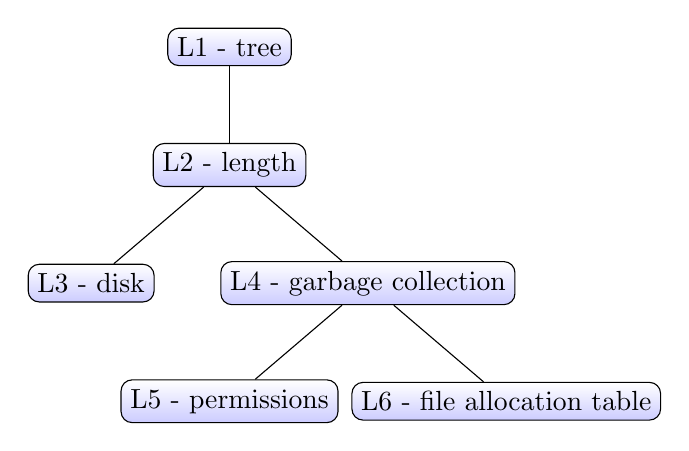
\begin{tikzpicture}[sibling distance=10em,
      every node/.style = {shape=rectangle, rounded corners,
        draw, align=center,
        top color=white, bottom color=blue!20}]
    \node {L1 - tree}
    child { node {L2 - length}
      child { node {L3 - disk}}
      child { node {L4 - garbage collection}
        child { node {L5 - permissions}}
        child { node {L6 - file allocation table}}}};
  \end{tikzpicture}
\end{frame}

\begin{frame}{Modelling a filesystem}
  \begin{itemize}
  \item \texttt{L1} filesystem representation: literal
    directory tree, in which non-leaf nodes represent (sub)directories
      and leaf nodes represent regular files
  \item \texttt{L4} filesystem representation:
    \begin{itemize}
    \item a tree, as above
    \item a disk, containing the textual contents of regular files
      broken into fixed-size blocks;
    \item and an allocation vector showing which blocks are in use
    \end{itemize}
  \item \texttt{L6} filesystem representation:
    \begin{itemize}
    \item a tree, as above
    \item a disk, as above
    \item and a file allocation table, mapping each block in a regular
      file to the next, forming a linked list which ends with a
      special value (EOC)
    \end{itemize}
  \end{itemize}
\end{frame}

\begin{frame}{L1 example}
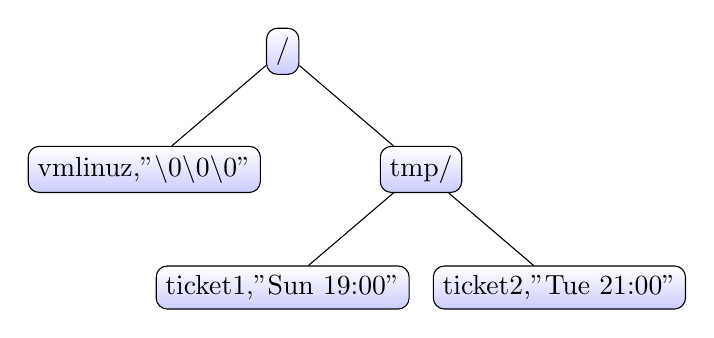
\begin{tikzpicture}[sibling distance=10em,
  every node/.style = {shape=rectangle, rounded corners,
    draw, align=center,
    top color=white, bottom color=blue!20}]
  \node {/}
    child { node {vmlinuz,{"}\textbackslash0\textbackslash0\textbackslash0{"}} }
    child { node {tmp/}
      child { node {ticket1,{"}Sun 19:00{"}}}
      child { node {ticket2,{"}Tue 21:00{"}}}};
\end{tikzpicture}
\end{frame}

\begin{frame}{L4 example}
  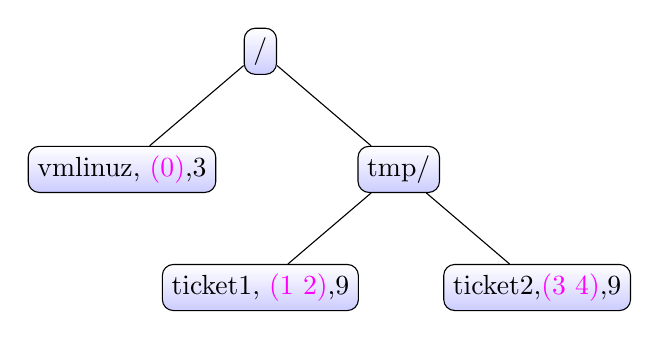
\begin{tikzpicture}[sibling distance=10em,
      every node/.style = {shape=rectangle, rounded corners,
        draw, align=center,
        top color=white, bottom color=blue!20}]]
      \node {/}
      child { node {vmlinuz, {\color[rgb]{1,0,1} (0)},3} }
      child { node {tmp/}
        child { node {ticket1, {\color[rgb]{1,0,1} (1 2)},9}}
        child { node {ticket2,{\color[rgb]{1,0,1} (3 4)},9}}};
  \end{tikzpicture}
  \begin{table}[]
    \centering
    \caption{Disk and allocation vector}
    \begin{tabular}{|l|l|l|}
      \hline
      {\color[rgb]{1,0,1} 0} & \textbackslash0\textbackslash0\textbackslash0   & true\\ \hline
      {\color[rgb]{1,0,1} 1} & Sun 19:0 & true\\ \hline
      {\color[rgb]{1,0,1} 2} & 0        & true\\ \hline
      {\color[rgb]{1,0,1} 3} & Tue 21:0 & true\\ \hline
      {\color[rgb]{1,0,1} 4} & 0        & true\\ \hline
      {\color[rgb]{1,0,1} 5} &          & false\\ \hline
    \end{tabular}
  \end{table}
\end{frame}

\begin{frame}{L6 example}
  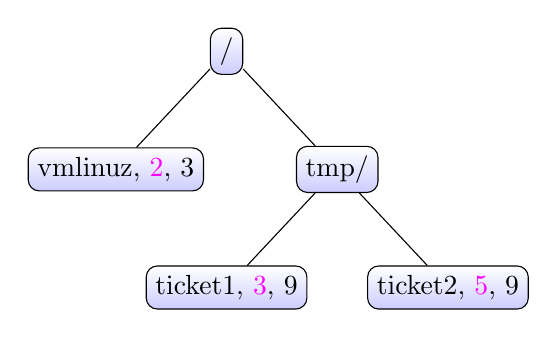
\begin{tikzpicture}[sibling distance=8em,
      every node/.style = {shape=rectangle, rounded corners,
        draw, align=center,
        top color=white, bottom color=blue!20}]]
      \node {/}
      child { node {vmlinuz, {\color[rgb]{1,0,1} 2}, 3} }
      child { node {tmp/}
        child { node {ticket1, {\color[rgb]{1,0,1} 3}, 9}}
        child { node {ticket2, {\color[rgb]{1,0,1} 5}, 9}}};
  \end{tikzpicture}
  \begin{table}[]
    \centering
    \caption{Disk and file allocation table}
      \begin{tabular}{|l|l|l|}
        \hline
        {\color[rgb]{1,0,1} 0} & & \\ \hline
        {\color[rgb]{1,0,1} 1} & & \\ \hline
        {\color[rgb]{1,0,1} 2} & \textbackslash0\textbackslash0\textbackslash0   & EOC\\ \hline
        {\color[rgb]{1,0,1} 3} & Sun 19:0 & 4\\ \hline
        {\color[rgb]{1,0,1} 4} & 0        & EOC\\ \hline
        {\color[rgb]{1,0,1} 5} & Tue 21:0 & 6\\ \hline
        {\color[rgb]{1,0,1} 6} & 0        & EOC\\ \hline
        {\color[rgb]{1,0,1} 7} &          & 0\\ \hline
      \end{tabular}
  \end{table}
\end{frame}

\begin{frame}{Conceptualising proofs}
  \begin{itemize}
  \item Initial focus on read-over-write properties (more details follow)
  \item Transition system formulation - filesystem instances
    (storing some files and directories with some metadata) become
    states, and file operations (reading, writing) become externally
    visible actions
  \item Small number of file operations, consistently named across
    models - \textit{stat, read, create, write, unlink}
  \item Refinement mappings - simply find functions that map each
    instance of a given model to an equivalent instance of a
    previously verified model
  \item Proof burden for \texttt{L1} (base model) - satisfaction of
    read-over-write properties
  \item Proof burden for \texttt{L2} (and following models) - mapping
    from \texttt{L2} instances to \texttt{L1} composes correctly with
    file operations in both \texttt{L2} and \texttt{L1}.
  \end{itemize}
\end{frame}

\section{The proofs}

\begin{frame}{Verifying the models}
  \begin{itemize}
  \item We've focussed so far on two filesystem properties, known in
    the literature as the \textit{read-over-write} properties.
    \begin{enumerate}
    \item After a write of some text at some location, a read of the
      same length at the same location should yield the text.
    \item After a write, a read at a different location should yield
      the same results as a read before the write.
    \end{enumerate}
  \item These properties have been proven for all models so far,
    including \texttt{L6}.
  \end{itemize}
\end{frame}

\begin{frame}{Proof example: first read-over-write in \texttt{L2}}
  \begin{figure}
    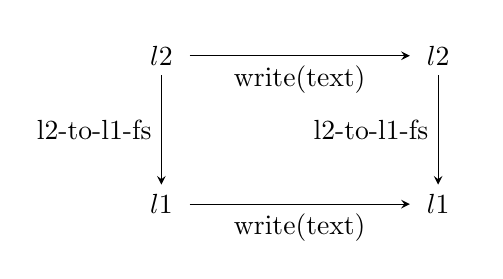
\begin{tikzpicture}
      \matrix (m) [matrix of math nodes,row sep=4em,column sep=8em,minimum width=2em]
              {
                l2 \pgfmatrixnextcell l2 \\
                l1 \pgfmatrixnextcell l1 \\};
              \path[-stealth]
              (m-1-1) edge node [left] {l2-to-l1-fs} (m-2-1)
              edge node [below] {write(text)} (m-1-2)
              (m-2-1.east|-m-2-2) edge node [below] {write(text)} (m-2-2)
              (m-1-2) edge node [left] {l2-to-l1-fs} (m-2-2);
    \end{tikzpicture}
    \caption{l2-wrchs-correctness-1}
  \end{figure}
  \begin{figure}
    \begin{tikzpicture}
      \matrix (m) [matrix of math nodes,row sep=4em,column sep=8em,minimum width=2em]
              {
                l2 \pgfmatrixnextcell text \\
                l1 \\};
              \path[-stealth]
              (m-1-1) edge node [left] {l2-to-l1-fs} (m-2-1)
              edge node [below] {read} (m-1-2)
              (m-2-1.east|-m-2-2) edge node [below] {read} (m-1-2);
    \end{tikzpicture}
    \caption{l2-rdchs-correctness-1}
  \end{figure}
\end{frame}

\begin{frame}{Proof example: first read-over-write in \texttt{L2}}
  \begin{figure}
    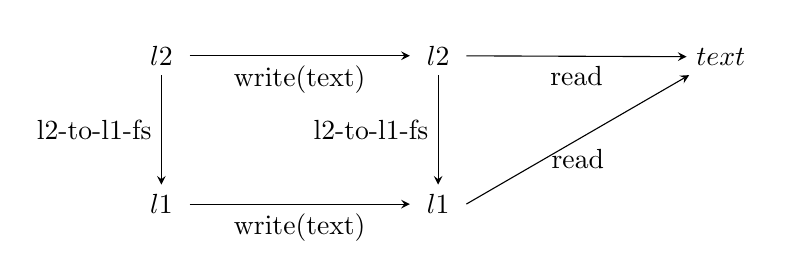
\begin{tikzpicture}
      \matrix (m) [matrix of math nodes,row sep=4em,column sep=8em,minimum width=2em]
              {
                l2 \pgfmatrixnextcell l2 \pgfmatrixnextcell text \\
                l1 \pgfmatrixnextcell l1 \\};
              \path[-stealth]
              (m-1-1) edge node [left] {l2-to-l1-fs} (m-2-1)
              edge node [below] {write(text)} (m-1-2)
              (m-2-1.east|-m-2-2) edge node [below] {write(text)} (m-2-2)
              (m-1-2) edge node [left] {l2-to-l1-fs} (m-2-2)
              edge node [below] {read} (m-1-3)
              (m-2-2.east) edge node [below] {read} (m-1-3);
    \end{tikzpicture}
    \caption{l2-read-over-write-1}
  \end{figure}
\end{frame}

\begin{frame}{Proof challenges}
  \begin{itemize}
  \item Invariant choice vital - core of the proof
  \item Define a "good state" of a filesystem, from which reading,
    writing and other operations can be safely carried out
  \item Do we make it simple, to help with verification? Do we make it
    general, to model as many real-world situations as possible?
  \end{itemize}
\end{frame}

\begin{frame}{Some choices}
  For our invariants, we choose to require:
    \begin{itemize}
    \item that each block on the disk is attributed to at most one
      regular file {\color[rgb]{0,0,1} (thus excluding hard links)}
    \item that the clusters attributed to each non-empty regular file
      end with a legal EOF value, as defined by the FAT specification
      {\color[rgb]{0,0,1} (thus excluding a class of errors)}
    \item that each regular file is annotated with "length", a
      metadata field that corresponds to the actual length of the file
      as determined by traversing the file allocation table and
      reading the corresponding blocks {\color[rgb]{0,0,1} (thus
        adding an extra field of metadata)}
    \end{itemize}
\end{frame}

\begin{frame}{Where does verification effort go?}
  Some expectations while modelling and verifying a filesystem with external storage:
  \begin{itemize}
  \item Proving exact results about available space on the disk and
    whether or not a write operation will succeed
  \item Proving file operations do not result in ill-formed regular
    files or subdirectories
  \item Defining good abstractions for well-formedness of regular
    files and subdirectories, and structuring proof around these
    abstractions
  \item Proving some general lemmata about built-in functions and
    later making them compatible with other books
  \item "Proof hacking" to reduce the use of the proof builder, use
    fewer hints and auxiliary lemmata, and reduce certification time
  \end{itemize}
\end{frame}

\section{Future work, related work and conclusion}

\begin{frame}{Future work}
  \begin{enumerate}
  \item Complete the FAT32 model, by means of
    \begin{itemize}
    \item supporting variable cluster sizes,
    \item moving the file allocation table onto the disk, and
    \item moving all file and directory metadata from the tree to the
      disk.
    \end{itemize}
  \item Validate the model through co-simulation with the Linux kernel
    implementation.
  \item Model a more complex filesystem, for instance ext4, by
    re-using algorithms and proofs from the models built so far.
  \end{enumerate}
\end{frame}

\begin{frame}{Related work}
  \begin{itemize}
  \item FSCQ (Chen, 2016) - novel filesystem, proven
    safe against crashes using Coq, performs comparably to
    ext4.
  \item COGENT (Amani, 2016) - "verifying compiler" translates specs
    in a DSL to C implementations free of some classes of bugs.
  \item SibylFS (Ridge, 2015) - "executable specification" for
    filesystem validates or rejects filesystem traces across multiple
    OSes.
  \item Hyperkernel (Nelson, 2017) - xv6 microkernel implemented
    with system calls changed to make them constant-time; in return,
    verification burden becomes lightweight enough for Z3 SMT solver.
  \item Our work's distinct aim: model an existing filesystem (FAT32)
    faithfully and match the resulting disk image byte-to-byte.
  \end{itemize}
\end{frame}

\begin{frame}{Conclusion}
  \begin{itemize}
  \item FAT32-adjacent filesystem formalised with
    a binary compatible file allocation table
  \item Read-over-write properties proven by means of refinement
    through a series of models
  \end{itemize}
\end{frame}

\end{document}
